\section{Preliminary Evaluations} \label{sec:results}

The \methodname was trained using the database described in the previous section. We split the dataset into training (90\%) and validation (10\%) using a stratified multi-label approach. Therefore, the proportion of compliant/non-compliant requirements shown in Table \ref{tab:req-dist} is preserved across all the images in both training and validation sets. The FICV competition database is considered the test set, and all the reported results were computed on it.

\subsection{Performance Results}

Table \ref{tab:best-results} summarizes the best results by requirement among all the methods shown in Table \ref{tab:comp}. Also, it includes the results of \methodname for easy comparison. All methods were evaluated by the benchmark tool of the FICV competition. As can be seen, the proposed method has the best results in 9 out of 23 requirements of \icao standard. Thus, the proposed method has the highest amount of best results in terms of requirements. We can also notice that \methodname has low rejection rates, with only four requirements rejecting at most 0.4\% of the evaluated images. Such rejections represent the false negatives from the face detector used to preprocess input images.

% Please add the following required packages to your document preamble:
% \usepackage[table,xcdraw]{xcolor}
% If you use beamer only pass "xcolor=table" option, i.e. \documentclass[xcolor=table]{beamer}
\begin{table}[!tb]
\centering
\caption{Comparison of the \methodname against the best results reported in the literature and by private SDK tools (see Table \ref{tab:comp}). All methods were evaluated by the benchmark tool of FICV using the \ficvofficial dataset.}
\label{tab:best-results}
\begin{tabular}{ccrrrr}
\hline
 & \multicolumn{3}{c}{\textbf{\begin{tabular}[c]{@{}c@{}}Best of Literature/\\ Commercial SDK\end{tabular}}} & \multicolumn{2}{c}{\textbf{ICAONet}} \\ \hline
\textbf{Req. \#} & Method & \multicolumn{1}{c}{EER} & \multicolumn{1}{c|}{{\color[HTML]{9B9B9B} Rej.}} & \multicolumn{1}{c}{EER} & \multicolumn{1}{c}{{\color[HTML]{9B9B9B} Rej.}} \\ \cline{2-6} 
\textbf{08} & BioPass Face & 1.60 & {\color[HTML]{9B9B9B} 3.30} & 2.10 & {\color[HTML]{9B9B9B} 0.60} \\
\textbf{09} & HMAX & 10.00 & {\color[HTML]{9B9B9B} 0.16} & \textbf{5.40} & {\color[HTML]{9B9B9B} 0.00} \\
\textbf{10} & BioLab & 3.40 & {\color[HTML]{9B9B9B} 1.20} & 49.00 & {\color[HTML]{9B9B9B} 0.00} \\
\textbf{11} & BioPass Face & 1.90 & {\color[HTML]{9B9B9B} 0.00} & \textbf{1.70} & {\color[HTML]{9B9B9B} 0.00} \\
\textbf{12} & id3 & 2.90 & {\color[HTML]{9B9B9B} 0.00} & \textbf{1.20} & {\color[HTML]{9B9B9B} 0.00} \\
\textbf{13} & BioPass Face & 0.00 & {\color[HTML]{9B9B9B} 0.00} & 7.30 & {\color[HTML]{9B9B9B} 0.00} \\
\textbf{14} & SDK 2 & 0.00 & {\color[HTML]{9B9B9B} 0.00} & 29.00 & {\color[HTML]{9B9B9B} 0.00} \\
\textbf{15} & Parente et al. & {\color[HTML]{333333} 11.90} & {\color[HTML]{9B9B9B} 3.40} & 13.70 & {\color[HTML]{9B9B9B} 0.40} \\
\textbf{16} & id3 & 0.20 & {\color[HTML]{9B9B9B} 1.00} & 0.80 & {\color[HTML]{9B9B9B} 0.00} \\
\textbf{17} & BioTest & 3.70 & {\color[HTML]{9B9B9B} 7.90} & 8.40 & {\color[HTML]{9B9B9B} 1.30} \\
\textbf{18} & id3 & 9.10 & {\color[HTML]{9B9B9B} 6.90} & \textbf{4.60} & {\color[HTML]{9B9B9B} 0.20} \\
\textbf{19} & BioLab & 0.60 & {\color[HTML]{9B9B9B} 0.00} & 1.00 & {\color[HTML]{9B9B9B} 0.00} \\
\textbf{20} & id3 & 1.00 & {\color[HTML]{9B9B9B} 2.00} & 8.20 & {\color[HTML]{9B9B9B} 1.50} \\
\textbf{21} & BioLab & 2.30 & {\color[HTML]{9B9B9B} 0.20} & 3.30 & {\color[HTML]{9B9B9B} 0.00} \\
\textbf{22} & Andrezza et al. & 7.70 & {\color[HTML]{9B9B9B} 2.50} & \textbf{3.30} & {\color[HTML]{9B9B9B} 0.20} \\
\textbf{23} & BioPass Face & 1.80 & {\color[HTML]{9B9B9B} 1.20} & \textbf{0.40} & {\color[HTML]{9B9B9B} 0.00} \\
\textbf{24} & BioLab & 2.10 & {\color[HTML]{9B9B9B} 0.00} & \textbf{0.80} & {\color[HTML]{9B9B9B} 0.00} \\
\textbf{25} & HMAX & 0.00 & {\color[HTML]{9B9B9B} 0.00} & 9.50 & {\color[HTML]{9B9B9B} 0.00} \\
\textbf{26} & HMAX & 0.00 & {\color[HTML]{9B9B9B} 0.10} & 2.30 & {\color[HTML]{9B9B9B} 0.60} \\
\textbf{27} & id3 & 6.80 & {\color[HTML]{9B9B9B} 0.80} & \textbf{5.70} & {\color[HTML]{9B9B9B} 0.20} \\
\textbf{28} & Parente et al. & 1.20 & {\color[HTML]{9B9B9B} 0.50} & \textbf{0.00} & {\color[HTML]{9B9B9B} 0.00} \\
\textbf{29} & id3 & 0.60 & {\color[HTML]{9B9B9B} 0.40} & 2.30 & {\color[HTML]{9B9B9B} 0.00} \\
\textbf{30} & BioPass Face & 1.20 & {\color[HTML]{9B9B9B} 2.70} & 41.40 & {\color[HTML]{9B9B9B} 0.00} \\ \hline
\multicolumn{4}{r}{\textbf{mean (\%)}} & 8.80 & 0.22 \\
\multicolumn{4}{r}{\textbf{median (\%)}} & 3.30 & 0.00 \\
\multicolumn{4}{r}{\textbf{avg. time (s)}} & \multicolumn{2}{c}{2.7} \\
\multicolumn{4}{r}{\textbf{max. time (s)}} & \multicolumn{2}{c}{3.4} \\
\multicolumn{4}{r}{\textbf{memory (MB)}} & \multicolumn{2}{c}{306.1}
\end{tabular}
\end{table}

There are only three methods with public results published in the \fvcongoing: BioPass Face \citep{fvcVsoft}, BioTest \citep{fvcBioTest}, and id3 \citep{fvcICAOCompliance}. In comparison to them, we have the best results in 11 out of all 23 requirements. Therefore, the \methodname is also the method with the highest amount of best results in terms of requirements in the FICV competition. Additionally, the proposed method has the second-best Median EER (3.3\%).

In terms of performance, the \methodname takes on average 1.8 seconds per image according to the official benchmark results on the FICV competition of the \fvcongoing website. In comparison with methods that evaluate all requirements, the proposed method is the fastest. However, according to our benchmarks, almost 90\% of the \methodname running time is dominated by the face detector (1.6s on average), which is a preprocessing step. On the other hand, the architecture of the proposed network takes only 0.15s of this total time. Furthermore, since the FICV competition runs the benchmarks in CPU-only computers, our network could be even faster by using a GPU. In the future, we intend to change our face detector to a faster alternative so that our total time in CPU will be reduced even more.

To improve these results, two distinct approaches can be followed. First, our dataset quality can be improved by increasing (i) the number of images and (ii) the variability of patterns of some requirements (like hat/cap). Thereby, the network can learn more effective descriptors and decrease our EER in these requirements. Secondly, we may change the network or try other loss functions. For instance, we can test loss functions designed for multi-label classification problems, like the Contrastive Loss \cite{khosla2020supervised}.

\subsection{Network Visualization}

\begin{figure*}[ht]
\centering
\subfigure[PCA]{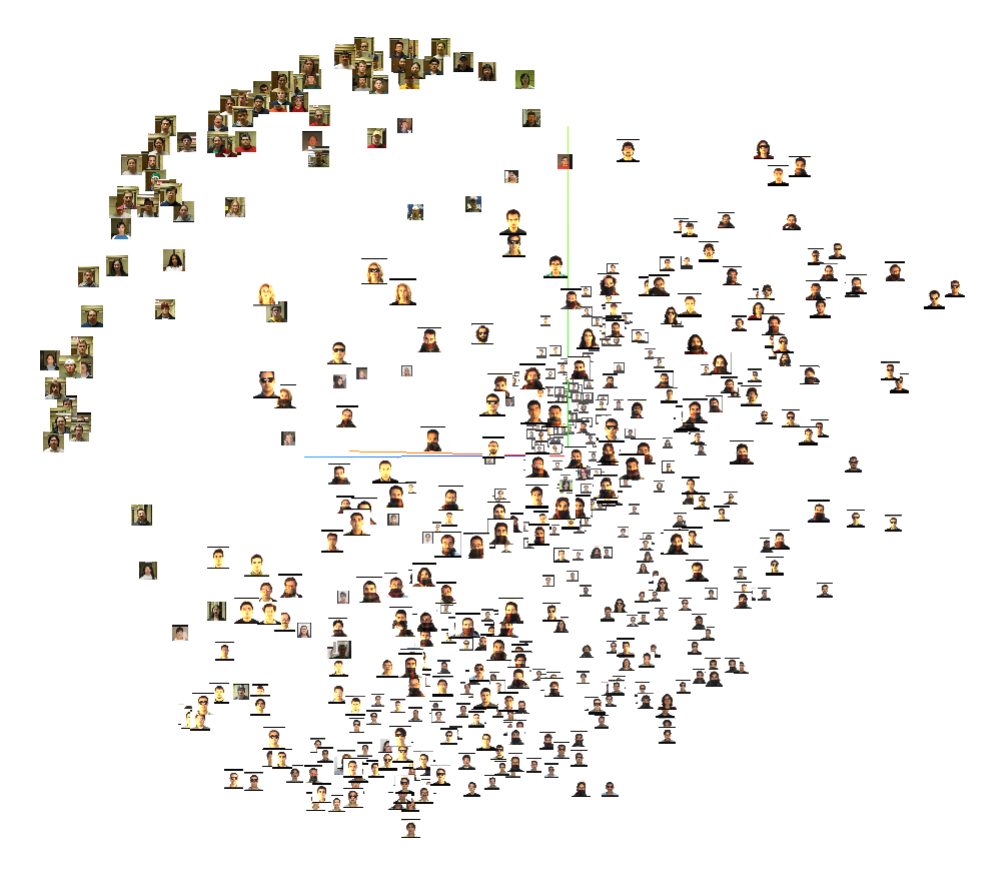
\includegraphics[width=0.4\linewidth]{images/pca.png}}
\hfill
\subfigure[t-SNE]{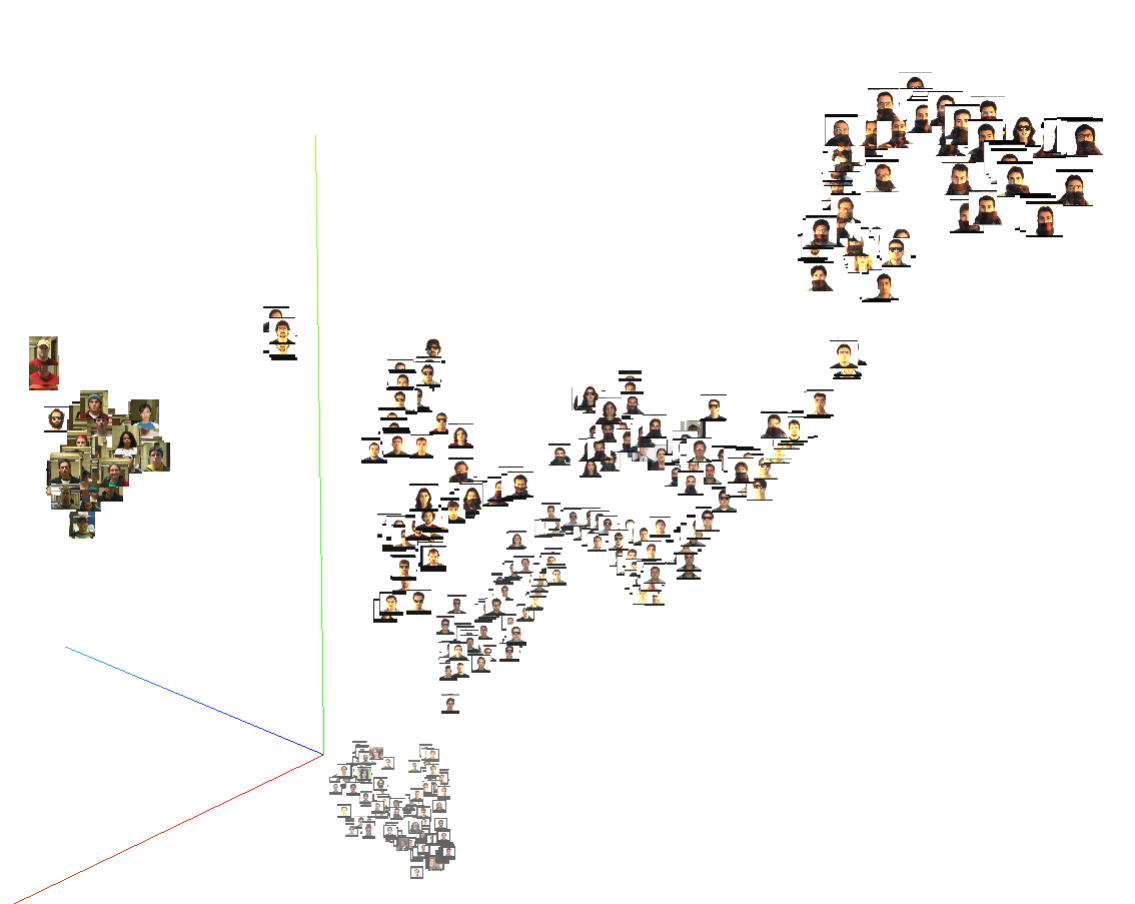
\includegraphics[width=0.4\linewidth]{images/tsne.png}}    
\caption{Visualization of the embeddings learned by \methodname. Original embeddings dimensions were reduced to 3D using (a) PCA and (b) t-SNE.}
\label{fig:embviz}
\end{figure*}

% um gráfico por linha

In addition to the performance results already presented, we decided to apply different techniques to understand the network outputs. First, we analyzed the embeddings learned by the network using algorithms for dimensionality reduction. Secondly, we applied network visualization techniques to understand which image regions are the most relevant according to each requirement. More details can be found in the next paragraphs.

A visualization of the embeddings learned by \methodname is shown in the 3D plots of Figure \ref{fig:embviz}. The embedding dimension was reduced to 3 dimensions and visualized via the PCA \citep{pca} and t-SNE \citep{tsne} methods using TensorBoard\footnote{https://www.tensorflow.org/tensorboard}. Each point in the plot is represented by a face image from the dataset. In the figure, it is possible to see the embeddings allow the formation of cluster-like regions containing face images that share the same semantic resemblance (e.g., varied background, sunglasses, unnatural skin tone, and veil over face). Although the figure shows only three dimensions, it is possible to observe that some dimensions are related to particular ICAO requirements. Such information is relevant to the multi-task classification branch of the \methodname architecture. 

Figure \ref{fig:shap} contains a visual representation of input images with local region contributions associated with each pose and photograph requirements. The SHAP \citep{shap2018} method was used to create that visualization. The figure provides evidence that the network learned useful representations for most of the requirements. In the fully compliant images (first three rows), the classification output is usually increased by the image regions related to that requirement. For example, in the eye-region dependent requirements (09, 15, 16, 20, 23, 24, and 26), the output is mainly influenced by regions closer to the eyes. Similar behaviors can be observed in requirements related to the mouth (28 and 29), skin (11, 19, 22), and the image aspect (08, 12, 13). 

However, we can notice the network was not able to learn relevant patterns in some requirements like \citeReq{\inkmarked}, \citeReq{\pixelation}, \citeReq{\framestooheavy}, \citeReq{\hatcap}, and \citeReq{\otherfacesortoys}. For requirements 10, 25, and 30, we believe the low amount of non-compliant images was the most crucial factor in contributing to the worst results of the proposed architecture, found in Table \ref{tab:req-dist}. In the case of \citeReq{\pixelation}, a possible cause for the high EER (42.7\%) could be the image resizing step applied in the input images. Finally, the random patterns in \citeReq{\hatcap} may show the variability of head props in our dataset must be insufficient to distinguish them from other patterns. 

\begin{figure*}[ht]
    \centering
    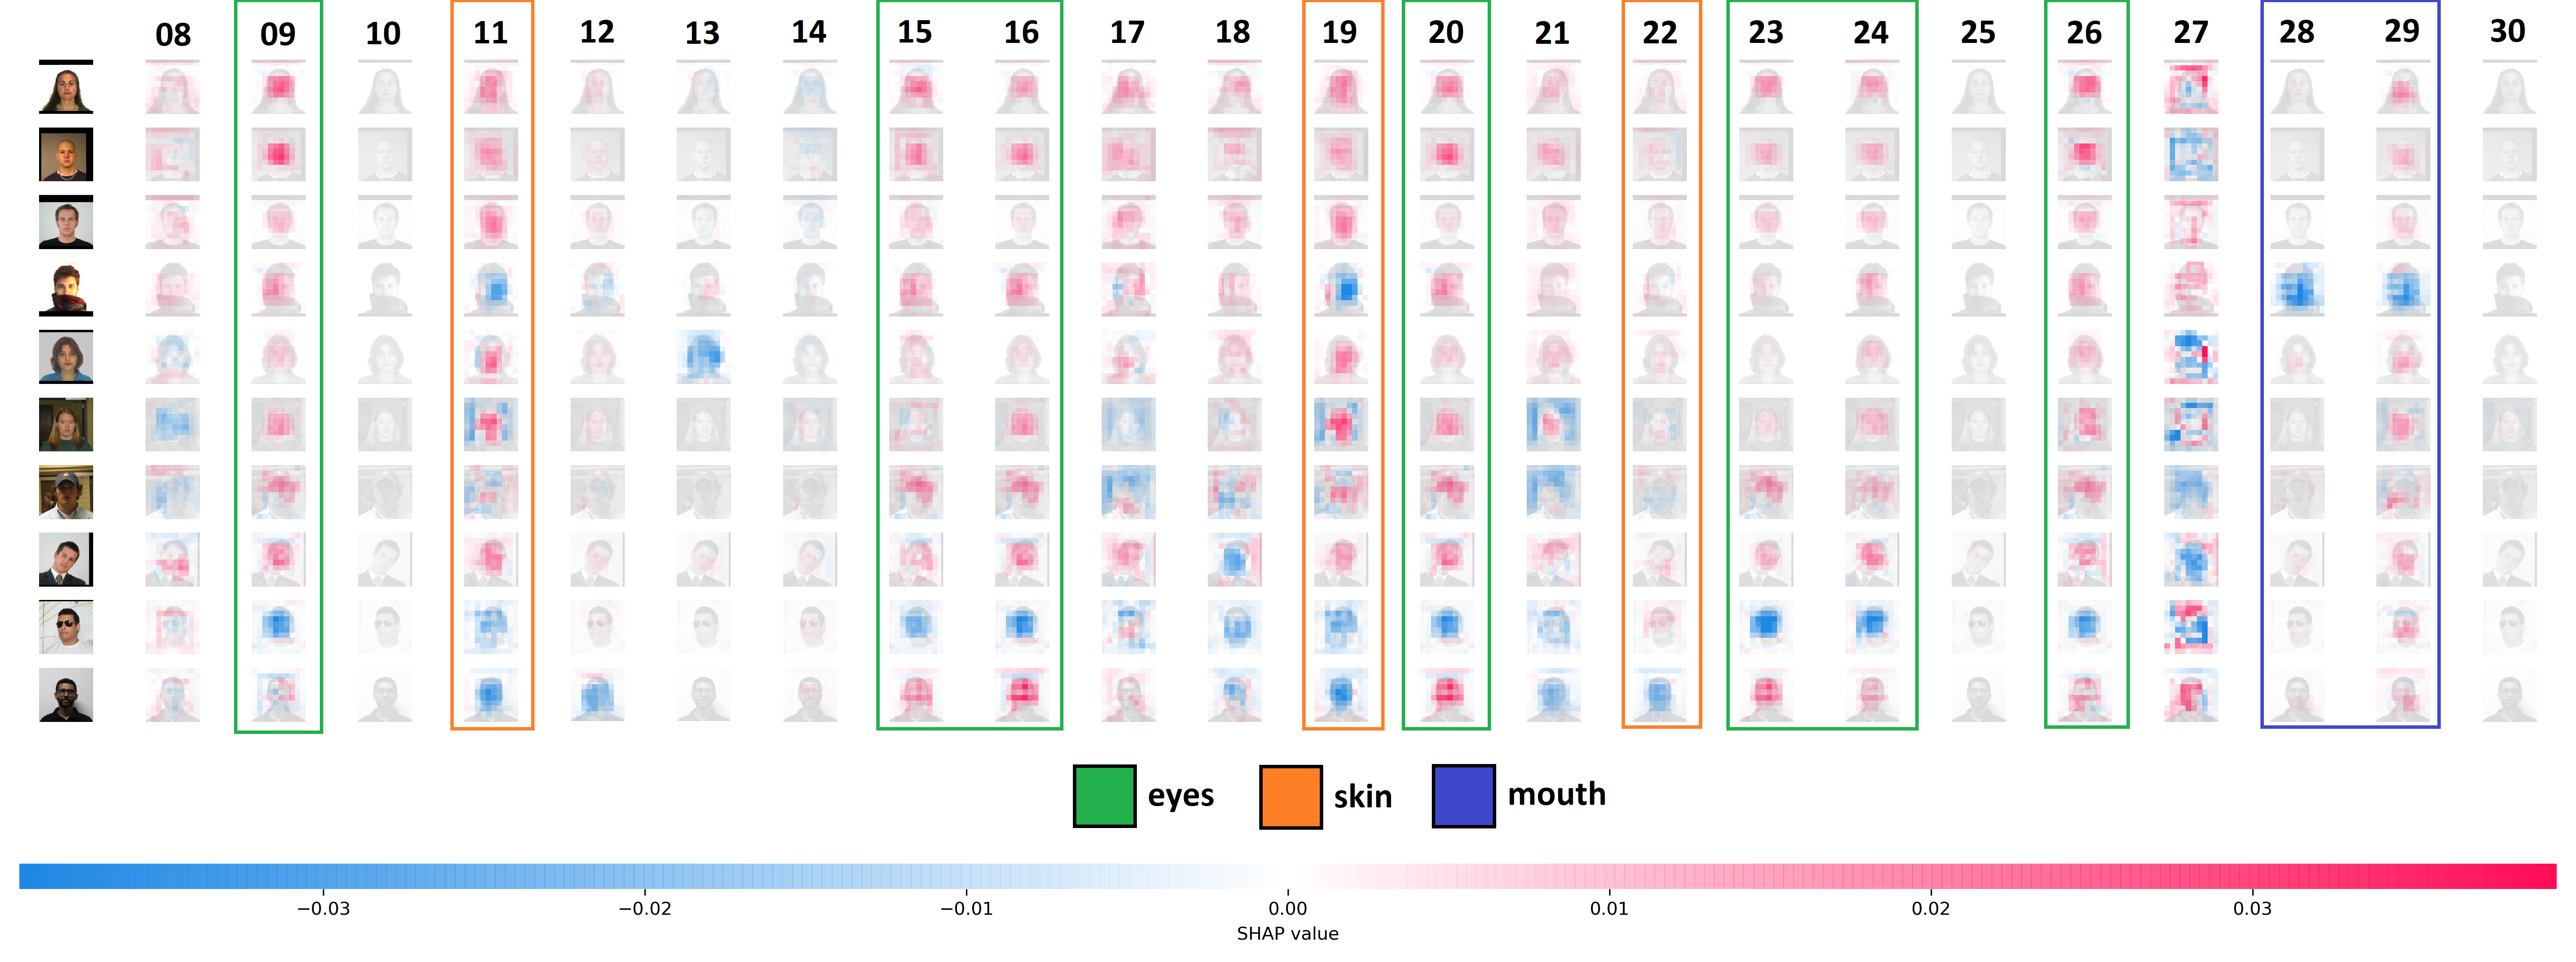
\includegraphics[width=\linewidth]{images/shap.png}
    \caption{Visual explanation of \methodname's output using SHAP. The first three images of the first column represent fully-compliant images from AR, FRGC, and PUT databases. The remaining rows are composed of images with at least one non-compliant requirement. The higher the SHAP value, the higher the compliance level for that requirement, and vice-versa. SHAP values near zero (white regions) means no contribution.}
    \label{fig:shap}
\end{figure*}

% We have already performed tests with one-shot learning approaches (like Siamese Networks) and triplet loss, but the results were worst than the proposed method. 
